\documentclass{article}
\usepackage[utf8]{inputenc}
\usepackage[a4paper, total={6in, 8in}]{geometry}

\usepackage{amsmath}
\usepackage{amssymb}
\usepackage{mathrsfs}
\usepackage{minted}
\usepackage[shortlabels]{enumitem}

% pakker for at lave bokse
\usepackage{blindtext}
\usepackage{tcolorbox}
\usepackage{graphicx}

\usepackage{minted}
\usepackage{subcaption}

\usepackage{hyperref}
\hypersetup{
  colorlinks   = true, %Colours links instead of ugly boxes
  urlcolor     = blue, %Colour for external hyperlinks
  linkcolor    = black, %Colour of internal links
  citecolor   = lightgray %Colour of citations
}

\makeatletter
\newcommand\xleftrightarrow[2][]{%
  \ext@arrow9999{\longleftrightarrowfill@}{#1}{#2}}
\newcommand\longleftrightarrowfill@{%
  \arrowfill@\leftarrow\relbar\rightarrow}
\makeatother

\begin{document}
%%%%%%%%%%%%%%%%%%%%%%%%%%%%%%%%%%%%%%%%%%%%%%%%%%%%%%%%%%%%%%%%%%
%%%%%%%%%%%%%%%%%%%%%%%%%%%%%%%%%%%%%%%%%%%%%%%%%%%%%%%%%%%%%%%%%%
%Fill in the appropriate information below
\newcommand{\norm}[1]{\left\lVert#1\right\rVert}     
\newcommand\course{Distributed Systems}        % <-- course name   
\newcommand\hwnumber{4}                                   % <-- homework number
\newcommand\Information{XXX/xxxxxxxx}                     % <-- personal information
%%%%%%%%%%%%%%%%%%%%%%%%%%%%%%%%%%%%%%%%%%%%%%%%%%%%%%%%%%%%%%%%%%
%%%%%%%%%%%%%%%%%%%%%%%%%%%%%%%%%%%%%%%%%%%%%%%%%%%%%%%%%%%%%%%%%%
%Page setup
\begin{titlepage}
    \begin{center}
        \vspace*{3cm}
            
        \Huge
        \textbf{\course{}}
            
        \vspace{1cm}
        \huge
        P\hwnumber : Synchronization
            
        \vspace{1.5cm}
        \Large
        by\\
        Team 7
        
        \textbf{Asger Song Høøck Poulsen} (202106630)\\% <-- author
        \textbf{Firas Harbo Saleh} (202109174) % <-- author
        
            
        \vfill
        
        A \course{} \\Project
            
        \vspace{0.5cm}
            
        
\includegraphics[width=0.4\textwidth]{img/aarhus-university.png}
        \\
        
        \Large
        
        \today
            
    \end{center}
\end{titlepage}
\tableofcontents
\section{Introduction}
    In the expansive field of distributed systems, the current project embarks on an insightful journey to explore and elucidate the fundamental concepts of logical clock algorithms, specifically focusing on Lamport Timestamps and Vector Clocks. This project aims to design, implement, test, and compare these algorithms, emphasizing their ability to order events in a distributed system with accuracy and efficiency. 

    The core challenge of this project lies in the intricate analysis and optimization of two pivotal logical clock algorithms - Lamport Timestamps and Vector Clocks. Our focus is twofold: firstly, to ensure the correctness of event ordering, and secondly, to optimize the overhead in terms of time, space, and message complexities. The journey encompasses a thorough process that begins with a detailed understanding of the algorithms, followed by a robust implementation in Python. The project progresses with rigorous testing and evaluation, comparing these algorithms against each other and benchmarking them against the state of the art.

    Through meticulous research, development, and analytical scrutiny, this project endeavors to contribute a comprehensive understanding of these algorithms. It seeks to provide clear insights into their operational mechanics, effectiveness in distributed environments, and the potential areas where they can be applied or further developed.


\section{Methods and Materials}
\subsection{Lamport Timestamp}
  The concept of Lamport Timestamps, introduced by Leslie Lamport\cite{Lamport:1978}, serves as a cornerstone in the realm of distributed systems for establishing a partial ordering of events. At the heart of this algorithm lies a simple yet powerful idea: using logical clocks — counters that are not tied to physical time — to sequence events across different processes in a distributed environment.

  Lamport Timestamps operate on the principle that each process in a distributed system maintains its own logical clock. When an event occurs, be it a message send or receive, or an internal event, the clock is incremented. The elegance of this system is its relative simplicity and the minimal overhead it incurs, making it a foundational approach in the study of distributed systems.

  \subsubsection{Happens-before}
    To establish synchronization among logical clocks in distributed systems, Leslie Lamport introduced the fundamental concept of happens-before, a crucial relation in Lamport Timestamps. This relation, denoted by $a \rightarrow b$, defines a chronological order between two events, stating that event $a$ happens before event $b$. This relation is transitive, meaning that \(\forall a,b,c\) if $a \rightarrow b$ and $b \rightarrow c$, then $a \rightarrow c$. The happens-before relation is also irreflexive, meaning that \(\forall a\): $a \nrightarrow a$, and antisymmetric, meaning that \(\forall a,b\): $a \neq b$, if \(a \rightarrow b\) then $b \nrightarrow a$.

    The happens-before relation is used to establish a partial ordering of events in a distributed system. The ordering is established by comparing the timestamps of two events. If $a \rightarrow b$, then $C(a) < C(b)$, where $C(a)$ denotes the timestamp of event $a$. However, it is important to note that the converse, if $C(a) < C(b)$, then $a \nrightarrow b$, is not necessarily true. This is because the happens-before relation is a partial ordering, meaning that it is not necessarily true that $a \rightarrow b$ or $b \rightarrow a$. When it is the cast that $a \nrightarrow b$ and $b \nrightarrow a$, the two events are said to be concurrent.

  \subsubsection{Lamport Timestamp Algorithm}\label{sec:lamport_timestamp_algorithm}
    Considering the happens-before relation, Lamport Timestamps can be defined as follows: \textit{The timestamp of an event is the maximum of its own timestamp and the timestamps of all events that happen-before it, plus one.} This definition can be expressed as the following equation:
    \begin{equation}
      C(e) = max(C(e), C(e')) + 1
    \end{equation}
    where $C(e)$ denotes the timestamp of event $e$, and $C(e')$ denotes the timestamp of the event that happens-before $e$. This equation is used to update the timestamp of an event when it occurs. The timestamp of an event is initialized to zero, and is incremented by one when an event occurs. The timestamp of an event is also included in messages sent between processes, and is used to update the timestamp of the receiving process.

    Consider the following example, where three processes, $P_1$, $P_2$ and $P_3$, communicate with each other depcited in figure \ref{fig:lamport_timestamp}. The processes run on different machines, and each process has its own logical clock. The clocks run at different rates. $P_1$ is incremented by $2$ units, $5$ units in process $P_2$, and $10$ units in process $P_3$, respectively.
    \begin{figure}[h!]
      \centering
      \includegraphics[width=0.6\textwidth]{img/lamport_timestamp.png}
      \caption{(a) Three processes, each with its own (logical) clock. The clocks run at different rates. (b) Lamport's algorithm synchronizes the clocks.}
      \label{fig:lamport_timestamp}
    \end{figure}

    The first example in figure \ref{fig:lamport_timestamp} shows the clocks of the three processes. Consider message $m_3$ which leaves $P_2$ at $80$ and arrives at $P_2$ at $40$. Similarly, $m_4$ from $P_2$ to $P_1$ leaves at $50$ and arrives at $22$. These values are clearly impossible in a real system, as the clocks are not synchronized. This is where Lamport Timestamps come into play.
    The second example shows the clocks after the Lamport Timestamp algorithm has been applied. The algorithm follows the happens-before relation to synchronize the clocks. Since $m_3$ left at $80$, it must arrive at $81$ or later. To ensure this, each message carries the sending time according to its sender's clock.

    To implement the Lamport Timestamp algorithm, each process maintains a local counter $C_i$ which are updated according to the following steps\cite{Raynal-Singhal:1996}:
    \begin{enumerate}
      \item When a process $P_i$ sends a message, it increments its counter $C_i$ by one, and attaches the new value to the message.
      \item When a process $P_i$ receives a message, it sets its counter $C_i$ to the maximum of its current value and the value in the received message, and increments its counter by one.
      \item When a process $P_i$ experiences an internal event, it increments its counter $C_i$ by one.
    \end{enumerate}

  \subsubsection{Overhead}
    The Lamport Timestamp algorithm incurs a minimal overhead in terms of time, space, and message complexities. The time complexity is $O(1)$, as the timestamp of an event is updated in constant time. The space complexity is $O(n)$, where $n$ is the number of processes in the distributed system, as each process maintains a single counter. The message complexity is also $O(n)$, as each message must carry the timestamp of the sending process.

  \subsection{Vector Clocks}
    Vector Clocks extend the concept of Lamport Timestamps, providing a refined approach to event ordering in distributed systems. Unlike Lamport Timestamps, which offer a partial ordering, Vector Clocks allow for a comprehensive understanding of causal relationships between events.

    \subsubsection{Principles and Operation}\label{sec:vector_clocks}
    In Vector Clocks, each process maintains an array of counters, one for each process, to track events across the distributed system. These arrays, known as Vector Clocks, are updated based on specific rules for different event types:
    \begin{enumerate}
    \item \textbf{Internal Events}: Increment the process's own counter.
    \item \textbf{Message Sending}: Increment the process's counter and attach the updated Vector Clock to the message.
    \item \textbf{Message Reception}: Update each counter to the maximum of the current value and the received value, then increment the process's own counter.
    \end{enumerate}
    
    \subsubsection{Causal Ordering}
    Vector Clocks enable determining causal relationships between events. An event $A$ is causally before event $B$ if $A$'s Vector Clock values are less than or equal to $B$'s, with at least one value being strictly less. Concurrent events are identified when neither event causally precedes the other.

    \subsubsection{Overhead}
    Vector Clocks incur a higher overhead than Lamport Timestamps, as each process must maintain an array of counters, one for each process in the distributed system. This results in a space complexity of $O(n^2)$, where $n$ is the number of processes in the system. The message complexity is also higher, as each message must carry the entire Vector Clock of the sending process. However, the time complexity is the same as Lamport Timestamps, as the Vector Clocks are updated in the same manner.

  \subsection{Development and Environment Tools}
    The implementation of the Lamport Timestamp algorithm and vector clocks was done using the following tools and technologies:
    \begin{itemize}
        \item \textbf{Git}: Git is a distributed version control system for tracking changes in source code during software development. It was used to manage the source code of the fortune cookie service and the Bully algorithm implementation.
        \item \textbf{GitHub}: GitHub is a web-based hosting service for version control using Git. It was used to host the source code of the fortune cookie service and the Bully algorithm implementation.
        \item \textbf{Visual Studio Code}: Visual Studio Code is a source-code editor. It was used to write the source code of the fortune cookie service and the Bully algorithm implementation.
        \item \textbf{Pytest}: Pytest is a testing framework for Python. It was used to write and run unit tests for the Bully algorithm implementation.
      \end{itemize}

\section{Experiments, Results and Discussion}
  This section presents the experimental setup, results, and a detailed discussion of the findings. The experiments were designed to test the accuracy, efficiency, and scalability of Lamport Timestamps and Vector Clocks in various distributed system scenarios.

  \subsection{Implementations}
    This subsection details the implementation of Lamport Timestamps and Vector Clocks, including the design and architecture of the class implementations.
    
    \begin{figure}[h!]
      \centering
      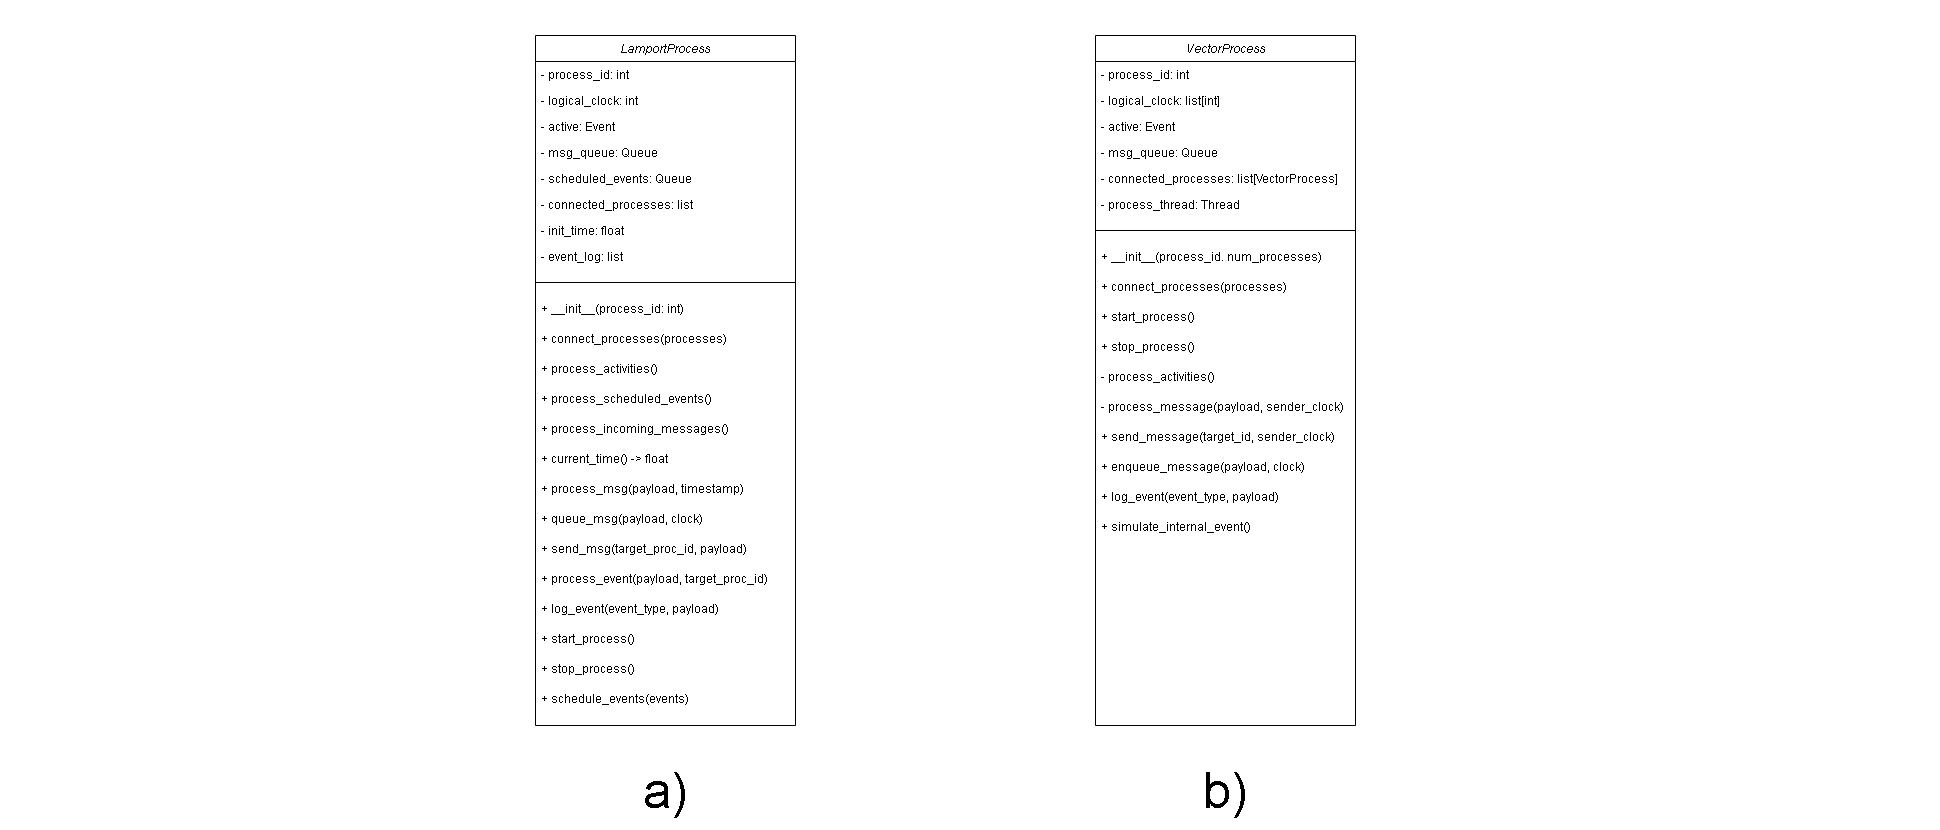
\includegraphics[width=\textwidth]{img/class_diagram.png}
      \caption{(a) UML class diagram of the Lamport Timestamp implementation. (b) UML class diagram of the Vector Clock implementation}
      \label{fig:class_diagram}

    \end{figure}
    \subsubsection{Lamport Timestamp}
      The Lamport Timestamp algorithm's implementation is encapsulated within the \texttt{LamportProcess} class, representing individual processes in a distributed environment. Figure \ref*{fig:class_diagram}a depicts the class diagram of the implementation.
      
      
      This class is equipped with a \texttt{logical\_clock} attribute, maintaining the current state of each process's logical clock. Core functionalities of the Lamport Timestamp algorithm are methodically distributed across three key methods: \texttt{send\_message} for managing outgoing messages, \texttt{process\_event} for internal event handling, and \texttt{process\_msg} for processing incoming messages. These methods collectively ensure the proper incrementation of the logical clock and adherence to the principles of the Lamport Timestamp algorithm. By following the steps outlined in \ref*{sec:lamport_timestamp_algorithm}, the following implementations of the main methods were developed:
      \begin{figure}[h!]
        \centering
        \begin{subfigure}{0.51\textwidth}
        \begin{minted}[fontsize=\scriptsize, linenos]{python}
def process_msg(self, payload, timestamp):
    """
    Process a received message, updating the logical clock.
    Args:
        payload: The message payload.
        timestamp: The timestamp of the received message.
    """
    self.logical_clock = max(timestamp, self.logical_clock) + 1
    self.log_event("Received", payload)
        \end{minted}
        \caption{process\_msg method}
        \label{fig:process_msg}
    \end{subfigure}
    \hfill
    \begin{subfigure}{0.51\textwidth}
        \begin{minted}[fontsize=\scriptsize, linenos]{python}
def send_msg(self, target_proc_id, payload):
    """Send a message to a target process."""
    if 0 <= target_proc_id < len(self.connected_processes):
        self.logical_clock += 1
        self.connected_processes[target_proc_id].queue_msg(payload, self.logical_clock)
        self.log_event("Sent", payload)
    else:
        self.log_event("Error", f"Invalid target process ID: {target_proc_id}")
        \end{minted}
        \caption{send\_msg method}
        \label{fig:send_msg}
    \end{subfigure}
    \par\bigskip % add some space
    \begin{subfigure}{0.51\textwidth}
        \begin{minted}[fontsize=\scriptsize, linenos]{python}
def process_event(self, payload, target_proc_id):
    """Process an event, either local or sending a message."""
    if payload == "STOP":
        self.active.set()
        return
    if target_proc_id == self.process_id:
        self.logical_clock += 1
        self.log_event("Local", payload)
    else:
        self.send_msg(target_proc_id, payload)
        \end{minted}
        \caption{process\_event method}
        \label{fig:process_event}
    \end{subfigure}
    \caption{Key methods of the LamportProcess class}
    \label{fig:lamport_process_methods}
    \end{figure}
      
    By meticulously handling the synchronization and ordering of events, the \texttt{LamportProcess} class serves as a testament to the algorithm's utility in distributed system design. Its implementation not only aligns with the theoretical underpinnings of Lamport Timestamps but also demonstrates their practical adaptability and scalability in complex distributed architectures.

    \subsubsection{Vector Clock}
      The implementation of Vector Clocks is effectively realized through the \texttt{VectorProcess} class, embodying each node in a distributed system. A visual representation of the implementation, including the class and sequence diagram, is illustrated in Figure \ref*{fig:class_diagram}b.
      
      
      This class maintains a \texttt{logical\_clock}, a list, that holds the logical time for each process in the system. Key operations of this implementation are encapsulated in methods such as \texttt{send\_message}, \texttt{process\_message}, and \texttt{simulate\_internal\_event}. These methods are designed to manage the synchronization and update of vector clocks during various types of events, including message sending, receiving, and internal events.
      By following the principles described in \ref*{sec:vector_clocks}, the following implementations of the main methods were developed:
      \begin{figure}[h!]
        \centering
        \begin{subfigure}{0.51\textwidth}
        \begin{minted}[fontsize=\scriptsize, linenos]{python}
def process_message(self, payload, sender_clock):
    """Update vector clock by comparing with the sender's clock"""
    for i in range(len(self.vector_clock)):
        self.vector_clock[i] = max(self.vector_clock[i], sender_clock[i])
    self.vector_clock[self.process_id] += 1
    self.log_event("Received", payload)
        \end{minted}
        \caption{process\_message method}
        \label{fig:process_message}
    \end{subfigure}
    \hfill
    \begin{subfigure}{0.51\textwidth}
        \begin{minted}[fontsize=\scriptsize, linenos]{python}
def send_message(self, target_id, payload):
    if target_id < len(self.connected_processes):
        self.vector_clock[self.process_id] += 1
        self.connected_processes[target_id].enqueue_message(payload, self.vector_clock.copy())
        self.log_event("Sent", payload)
        \end{minted}
        \caption{send\_message method}
        \label{fig:send_message}
    \end{subfigure}
    \par\bigskip % add some space
    \begin{subfigure}{0.51\textwidth}
        \begin{minted}[fontsize=\scriptsize, linenos]{python}
def simulate_internal_event(self):
    """Simulate an internal event for the current process."""
    self.vector_clock[self.process_id] += 1
    self.log_event("Internal Event", "Internal event occurred")
        \end{minted}
        \caption{simulate\_internal\_event method}
        \label{fig:simulate_internal_event}
    \end{subfigure}
    \caption{Key methods of the VectorProcess class}
    \label{fig:vector_process_methods}
\end{figure}

      The \texttt{VectorProcess} class demonstrates a simple approach of Vector Clocks in maintaining a causal relationship among distributed processes. It highlights the ability of Vector Clocks to not only track event chronology like Lamport Timestamps but also to provide a deeper understanding of the causal dependencies among events. This enhanced capability makes Vector Clocks a more robust solution for certain complex scenarios in distributed systems.
      


    \subsection{Test Scenarios and Methodology}
      This subsection outlines the specific scenarios and methodologies applied to test the Lamport Timestamp and Vector Clock implementations. The aim was to rigorously evaluate their correctness with respect to the theoretical underpinnings of the algorithms.
      
      \subsubsection{Testing Framework}
      The testing was conducted using the Python-based Pytest framework, which provided a robust and flexible environment for creating and executing a comprehensive set of test cases. Each logical clock algorithm was subjected to a series of tests designed to prove its correctness. All test cases are included in the \texttt{test\_logical\_clocks.py}-file. Figure (missing) illustrates some of the test cases implemented.
      
      For both implementations, tests were designed to validate the correctness of logical clock increments during internal events, message sending, and message receiving. Key scenarios included:
      \begin{itemize}
          \item \textbf{Local Event Handling:} Testing how the logical clock is incremented during internal events within a process.
          \item \textbf{Message Sending:} Assessing the behavior of the logical clock when a process sends a message to another process.
          \item \textbf{Message Reception:} Evaluating the logical clock's update upon receiving a message..
      \end{itemize}
      
   
  \subsection{Results}

    Present the results of your experiments in a clear and structured manner. This could include tables, graphs, or charts that effectively convey the data collected during testing.

  \subsection{Discussion}

    Analyze the results, discussing how they meet the objectives set out at the beginning of the project. Highlight any interesting or unexpected findings, and how they impact the understanding of Lamport Timestamps and Vector Clocks in distributed systems. Discuss any patterns or trends observed in the data, and what they signify about the algorithms' performance and reliability.

  \subsection{Limitations of the Study}

    Acknowledge any limitations encountered in your experimental setup or methodology, and how these might affect the interpretation of the results.

  \subsection{Implications of Findings}

    Discuss the broader implications of your findings, both for theoretical research and practical applications in distributed systems.

\section{Conclusion and perspectives}
    \subsection{Conclusion}
    
    \subsection{Lessons Learned}
      Partial ordering vs total ordering

    \subsection{Future Work}

\newpage
    \bibliographystyle{IEEEtran} % We choose the "plain" reference style
    \nocite{*}
    \bibliography{P4} % Entries are in the refs.bib file
\end{document}